\chapter{Herramientas y Software}
\label{chap:hs}
En este capítulo se explican las herramientas y librerías utilizadas para llevar a cabo el proyecto.
\section{Lenguajes de programación}
    \subsection{C++}    
El proyecto se desarrollo en su totalidad en C++. Esto se debe a que como se menciona previamente, este trabajo forma parte del esfuerzo académico de \citeauthor{IglesiasGuitian2022} y por coherencia se decidió seguir la línea de trabajo.
C++ es un lenguaje de programación que se beneficia de programación orientada a objetos sobre la sintaxis de C y ha utilizado para implementar librerías gráficas intrínsecas en el proyecto.

\section{Sistema Operativo}
\subsection{Windows 11}
Windows 11 es un sistema operativo desarrollado por  © Microsoft. Se utilizó debido a la familiaridad del proyecto con el mismo.
\section{Control de versiones}
    \subsection{GitLab}
Para llevar a cabo el control de versiones se utilizó GitLab ya que el código implementado formaba parte de le proyecto previamente mencionado, y este se almacena en GitLab.
\section{Entorno de desarrollo}
    \subsection{Visual Studio Community}
Es el Entorno de desarrollo de C++ por excelencia en Windows.
\section{Herramientas}
    \subsection{\acrfull{dicom}}
    \acrshort{dicom} es la denominación de un estándar utilizado principalmente para la visualización, impresión, almacenamiento y transmisión de imágenes y datos de propósito médico.
    Los ficheros \acrshort{dicom} consisten en una cabecera con campos estandarizados y de forma libre, y un cuerpo con datos de imagen. Un objeto \acrshort{dicom} simple puede contener solamente una imagen, pero esta imagen puede tener múltiples fotogramas, permitiendo el almacenamiento de bloques de datos con varios fotogramas.
   
    \subsection{3D Slicer}
3D Slicer es un programa de software libre diseñado para solventar los problemas mas avanzados de la computación de imagen relacionados con las aplicaciones clínicas y biométricas. Las capacidades del mismo se encuentra la  posibilidad de implementar scripts de python, segmentación de imágenes y volúmenes, la posibilidad de añadir extensiones para aumentar su funcionalidad y la interoperabilidad del estándar \acrshort{dicom} entre otras.

\subsection{Meshmixer}
Al procurar generar un modelo a partir de una nube de puntos de un TAC, es común encontrarse con que los modelos exportados en STL contienen errores y no pueden ser impresos directamente. Se probaron varias herramientas para solventar estos errores en la estructura de los modelos 3D, pero finalmente Meshmixer (https://www.meshmixer.com) resultó dar los mejores resultados a la hora de arreglar las geometrías con esta casuística can específica.
    \subsection{Blender}
Blender es la herramienta de software libre para la creación 3D por excelencia.
    \subsection{UltiMaker Cura}
UltiMaker Cura es el programa desarrollado por UltiMaker para generar el GCODE necesario para imprimir modelos en una impresora de dicha marca. Se utilizó ya que permite importar ajustes específicos de la impresora sobre la que se trabajo de forma sencilla.
\section{Frameworks}
\subsection{OpenXR}
OpenXR es una \acrfull{api} multi plataforma, que permite el desarrollo de medios en el \textit{virtual continuum} mediante ordenadores a través de interacción  humano-máquina.
Esta \acrshort{api} es la interfaz con un runtime para llevar a cabo operaciones comunes como puede ser acceder al estado de un mando o periférico, obtener o predecir la posicion del sistema o enviar frames para ser renderizados.
\paragraph{}

\subsubsection{Ciclo de Vida}
En \ref{fig:openxrlifecycle} se muestra la máquina de estados de la sesión:
\begin{enumerate}
    \item La aplicación crea una sesión escogiendo un sistema y una API gráfica. En un primer momento esta se encuentra en estado IDLE.
    \item Se monitorea la sesion en busca de cambios de estados mediante eventos.
    \item Cuando el runtime determina que el sistema esta listo para empezar con el contenido \acrshort{xr} de la sesion, se recibe un cambio de estado a READY.
    \item Mientras que la sesión esta corriendo, se espera que la aplicación ejecute continuamente el frame loop, estableciendo así sincronización con el runtime, lo que provoca un cambio de estado a SYNCHRONIZED.
    \item Una vez que el runtime este listo para mostrar frames de la aplicación, se notifica con el estado VISIBLE.
    \item Si el runtime detecta que es posible recibir entradas desde un mando, reconocimiento facial o demás, notifica con un estado FOCUSED.
    \item Estos estados como se ve en \ref{fig:openxrlifecycle} también tienen carácter retroactivo, de forma que cuando las características dejan de estar disponibles se va cambiando de estado, hasta que se desee parar o cerrar la aplicación.
    
\end{enumerate}


\begin{figure}[hp!]
  \centering
  \includegraphics[width=1.0\textwidth]{imaxes/openXR_life_cycle.png}
  \caption{Ciclo de vida de OpenXR.}
  \label{fig:openxrlifecycle}
\end{figure}
\paragraph{}

\subsubsection{API Layers}
OpenXR esta diseñado como una \acrshort{api} por capas, lo que quiere decir que una aplicacion puede insertar más o menos capas entre la aplicación y la implementación del runtime seleccionada. Estas capas proveen de funcionalidades adicionales interceptando las funciones de OpenXR de la capa superior, y posteriormente llevando a cabo operacione distinas a las que se llevarian a caboen caso de que no estuviese presente la capa. En el mas sencillo de los casos una capa simplemente llama a la inferior con los mismos argumentos, pero en casos mas elaborados se pueden implementar funcionalidades no dusponibles en las capas o incluso runtime inferiores \ref{fig:openxrapilayer}.
\paragraph{}
Esta arquitectura permite el desarrollo multiplataforma con mayor simplicidad, pero es dependiente de que los vendedores implementen sus propias capas API de OpenXR, lo que limita en ciera medida las 


\begin{figure}[hp!]
  \centering
  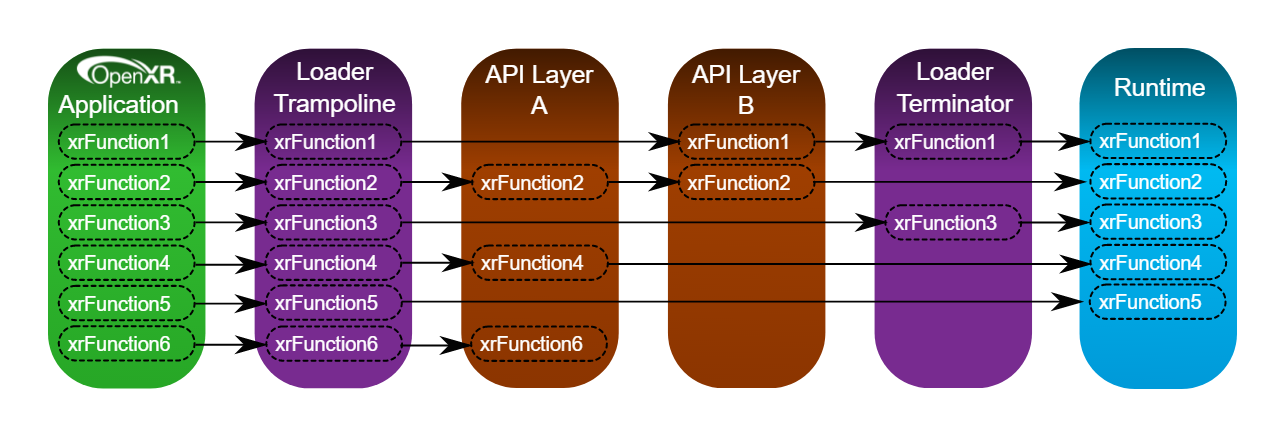
\includegraphics[width=1.0\textwidth]{imaxes/openxr_api_layer_graph.png}
  \caption{Explicación de la API por capas.}
  \label{fig:openxrapilayer}
\end{figure}

\subsection{OpenCV}
\acrfull{opencv} es una librería de código abierto que implementa principalmente funciones de visión artificial en tiempo real. Se utilizó para la generación y el seguimiento de los marcadores ARuco que forma parte de los paquetes adicionales de la librería.
\subsection{ARuco}
Los últimos años, los desarrollos de nuevos marcadores han tendido a un cuadrado negro con distintos patrones interiores \ref{fig:qrtags}, ya que permiten extraer la pose de la cámara a partir de sus 4 esquinas, asumiendo que esta esté adecuadamente calibrada \cite{GarridoJurado2014}. Esencialmente estos marcadores comparten ciertas características comunes en cuanto a su funcionamiento, entre todas las opciones disponibles se escogió ArUco como solución a nuestro proyecto por varios motivos:
\begin{itemize}
    \item Diccionarios generados dinámicamente.
    \item Posibilidad de crear tablas de marcadores lo que incrementa la resistencia a las oclusiones.
    \item Software para la calibración de cámara: De forma sencilla se puede calibrar cualquier cámara.
    \item La librería ha soportado el paso de los años sin problema, existiendo ejemplos y documentación extensa sobre el funcionamiento de la misma, facilitando así el desarrollo.
\end{itemize}


\begin{figure}[hp!]
  \centering
  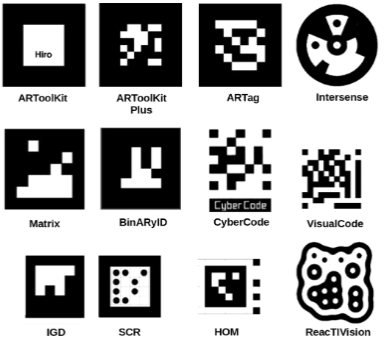
\includegraphics[width=0.75\textwidth]{imaxes/qrtags.png}
  \caption{Ejemplos de marcadores fiduciarios previos}
  \label{fig:qrtags}
\end{figure}

\subsection{Funcionamiento de Aruco}

\subsubsection*{Captura de imágenes o videos}
La captura de imágenes o vídeos se realiza mediante un dispositivo específico, como una cámara digital o un dispositivo móvil con cámara incorporada. En este paso se espera obtener una serie de imágenes o un vídeo sobre el que se espera encontrar uno o varios marcadores ARuco.
\subsubsection*{Conversión a escala de grises}
La conversión a escala de grises se realiza mediante el algoritmo de promedio ponderado de los canales RGB. Esta conversión reduce la cantidad de información a procesar y mejora la velocidad de procesamiento al trabajar con un único canal de información.
\subsubsection*{Aplicación de un filtro de bordes}
Para resaltar los bordes de los marcadores en la imagen se aplica un filtro de bordes. Un ejemplo común es el algoritmo de Canny, que se basa en la detección de gradientes y utiliza un umbral para determinar que bordes son relevantes y cuales no.
\subsubsection*{Detección de contornos}
Se utiliza un algoritmo de detección de contornos adaptativo para encontrar los contornos de los marcadores en la imagen. Un algoritmo común es el Transformada de Hough que permite detectar contornos circulares y lineales en la imagen. Este algoritmo busca patrones en la imagen que se correspondan con los contornos de los marcadores ARuco.
En un sistema de thresholding tradicional, se elige un umbral global para toda la imagen. Cualquier píxel con un valor de brillo superior al umbral se considera activo (p.ej. negro) y cualquier píxel con un valor de brillo inferior al umbral se considera inactivo (p.ej. blanco). Sin embargo, en muchas imágenes, el nivel óptimo de umbral puede variar entre diferentes partes de la imagen. El thresholding adaptativo se utiliza para solucionar este problema.

El thresholding adaptativo se divide en dos pasos:

Selección de una región de interés (ROI) en la imagen. Esta región puede ser de cualquier tamaño y forma.

Selección del umbral para cada pixel dentro de la ROI. El umbral se calcula a partir de la distribución de los niveles de gris dentro de la ROI.

Existen varios métodos para calcular el umbral adaptativo, algunos de los mas conocidos son:
\begin{itemize}
\item Método de media global
\item Método de la desviación estándar
\item Método de Otsu
\end{itemize}
Cada uno de estos métodos tiene sus propios pros y contras y en función de la aplicación y el tipo de imagen, se puede elegir uno u otro.
Además es posible modificar los siguientes parámetros para adecuar la librería a nuestro caso de uso, los más importantes son:
\begin{itemize}
    \item   \textbf{markerBorderBits:}
    El número de bits que se utilizan para representar el borde de un marcador. El borde de un marcador es el área blanca que rodea el patrón de código de barras en un marcador ARuco. El valor predeterminado es 4.
    \item \textbf{adaptiveThreshWinSizeMin and adaptiveThreshWinSizeMax:}
    El tamaño mínimo y máximo de la ventana utilizada para la umbralización adaptativa. La umbralización adaptativa es un método para determinar automáticamente el valor de umbral óptimo para una imagen. Estos parámetros se utilizan para especificar el tamaño de la ventana en píxeles que se utilizará para la umbralización adaptativa.
    \item \textbf{adaptiveThreshWinSizeMax:}
    Especificaa el paso o incremento con el cual se variará el tamaño de la ventana utilizada en la umbralización adaptativa.
    \item \textbf{adaptiveThreshConstant:}
    especificar una constante que se utilizará en el cálculo del valor de umbral para cada subregión de la imagen.
    \item \textbf{minMarkerPerimeterRate and maxMarkerPerimeterRate:}
    El porcentaje mínimo y máximo del perímetro de un marcador en relación con su área. Estos parámetros se utilizan para especificar el tamaño mínimo y máximo de los marcadores que se detectarán en la imagen.
    \item \textbf{minCornerDistanceRate:}
    La relación entre la distancia entre las esquinas de un marcador y su longitud de lado. Esto es utilizado para ignorar marcadores que tengan esquinas muy cercanas entre sí.
    \item \textbf{minDistanceToBorder:}
    La distancia mínima desde el borde de la imagen hasta el borde de un marcador. Esto se utiliza para ignorar marcadores que estén demasiado cerca del borde de la imagen.
    \item \textbf{ minMarkerDistanceRate:}
    La relación entre la distancia entre los marcadores y su longitud de lado. Esto se utiliza para ignorar marcadores que estén demasiado cerca entre sí.
\end{itemize}

\subsubsection*{Extracción de Bits}
Una vez que se han detectado los contornos de los posibles candidatos en una imagen, se analizan los bits extraídos de cada uno de estos para determinar si en efecto son marcadores o no.
Para ello se somete cada sección de la imagen a una corrección de perspectiva. A continuación se subdivide el candidato en la cantidad previamente establecida en el diccionario de bits que componen cada marcador. Dado que en un bit pueden encontrarse píxeles de los bits contiguos o errores en la imagen capturada por la cámara, se establece extrae el valor del bit en función de la desviación típica de los píxeles de dicho bit \ref{fig:mbe}.

\begin{figure}[hp!]
  \centering
  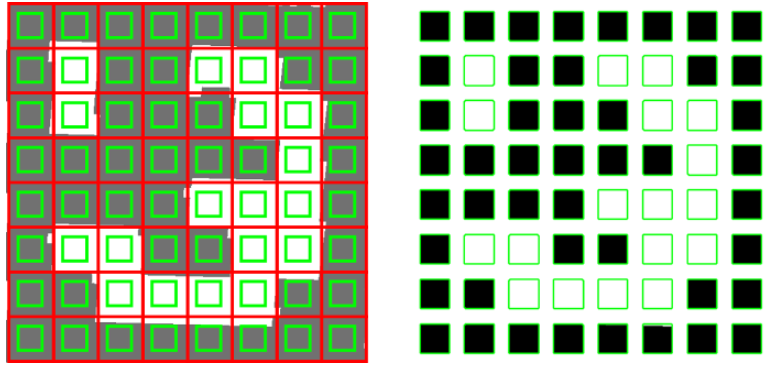
\includegraphics[width=0.85\textwidth]{imaxes/marker_bits_extraction.png}
  \caption{Proceso de extracción de Bits}
  \label{fig:mbe}
\end{figure}

\subsubsection*{Identificación de Marcadores}
Una vez determinados los bits de los que esta compuesto cada candidato a marcador es necesario determinar si el código extraído pertenece al diccionario y en caso de ser necesario aplicar algoritmos de corrección de errores.
La primera operación consiste en determinar la cantidad de bits erróneos permitidos en el borde de un marcador, ya que todos los marcadores ARuco cuentan al menos con un bit de borde. En lo que a corrección de errores se refiere, cada diccionario cuenta con un límite teórico de bits que pueden ser corregidos.

\subsubsection*{Refinado de Esquinas}
Una vez se han detectado e identificado todos los marcadores es posible realizar  un refinado a nivel de subpíxel de las esquinas para favorecer a la precisión del sistema. Este ultimo paso es altamente costoso a nivel computacional, pero se recomienda en aplicaciones en las que prima la precisión como es el caso.
\paragraph{}
Esta librería trabaja con un Pinhole Camera Model lo que quiere decir que se considera como el origen de coordenadas el punto en el que todos los rayos de lux convergerían en una supuesta cámara estenopeica ideal.

Las coordenadas se definen de la siquiente forma: Z crece frente a la camara mientras que X e Y se encuentran en el plano otrogonal de Z. X aumenta de derecha a izquierda e Y de abajo a arriba.




\begin{figure}[hp!]
  \centering
  
\includegraphics[width=0.3\textwidth]{imaxes/qr.png}
  \caption{Marcador Generado con ArUco}
  \label{fig:qr}
\end{figure}


\section{Hardware}
\subsection{Impresión 3D}
Se utilizaron dos impresoras 3D a lo largo del proyecto puesto que eran necesarios distintos requisitos para cada pieza.
Los modelos anatómicos debido a su complejidad se imprimieron en una impresora Fuse 1+ 30W que utiliza polvo de nylon para llevar a cabo las piezas.
Para los marcadores fiduciarios, se utilizo la Ultimaker 3, ya que se trata de figuras mas simples en las que la posibilidad de imprimir en distintos colores era especialmente importante.
\subsection{\acrfull{hmd}}
Para la implementación del sistema de captación de imagen y tracking se utilizó un casco HTC Vive Pro 2.

